\section{Calibrating the certificate}
\label{sec:calibration}

% GENERATED by make_paper_assets.py -- do not edit by hand.
\begin{figure}[t]
\centering
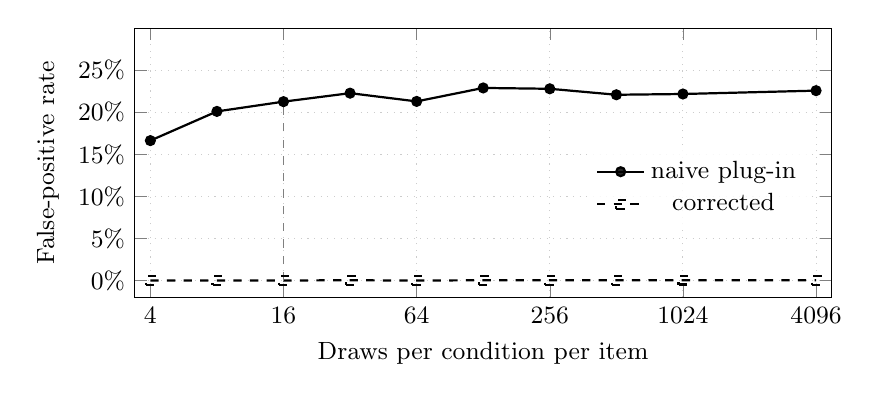
\begin{tikzpicture}
\begin{semilogxaxis}[
  width=0.86\columnwidth, height=5.0cm, log basis x=2,
  xlabel={Draws per condition per item}, ylabel={False-positive rate},
  xmin=3.4, xmax=4800, ymin=-0.02, ymax=0.30,
  ytick={0,0.05,0.1,0.15,0.2,0.25}, yticklabels={0\%,5\%,10\%,15\%,20\%,25\%},
  xtick={4,16,64,256,1024,4096}, xticklabels={4,16,64,256,1024,4096},
  legend style={at={(0.97,0.55)}, anchor=north east, font=\small, draw=none,
                fill=white, fill opacity=0.85, text opacity=1},
  grid=major, grid style={dotted, gray!40},
  tick label style={font=\small}, label style={font=\small},
]
\addplot[thick, mark=*, mark size=1.6pt] coordinates {(4,0.1664) (8,0.2011) (16,0.2127) (32,0.2228) (64,0.2130) (128,0.2290) (256,0.2280) (512,0.2209) (1024,0.2218) (4096,0.2258)};
\addlegendentry{naive plug-in}
\addplot[thick, dashed, mark=square, mark size=1.6pt] coordinates {(4,0.0000) (8,0.0000) (16,0.0001) (32,0.0004) (64,0.0000) (128,0.0004) (256,0.0003) (512,0.0003) (1024,0.0005) (4096,0.0003)};
\addlegendentry{corrected}
\draw[gray, dashed] (axis cs:16,-0.02) -- (axis cs:16,0.2127);
\end{semilogxaxis}
\end{tikzpicture}
\caption{False-positive rate of the compatibility certificate versus sampling
budget, under a null resampled from the real full-panel disclosure rates and
answer-law skew (8{,}000 replications per point, full grid in
Table~\ref{tab:calibration}). The dashed vertical marks the 16-draw budget used
throughout. The naive certificate does not approach zero with more data: it
plateaus at 21--23\% out to 4{,}096 draws, 256$\times$ our budget,
because near-total disclosure leaves no slack to absorb sampling noise. The
per-item corrected certificate (plotted) stays at or below 0.05\% (95\% upper bounds at most
0.13\%). The family-wise regime, used for the certified violations of Section~\ref{sec:models},
rejected none of the 8{,}000 replications at any draw count (Table~\ref{tab:calibration}).}
\label{fig:calibration}
\end{figure}


\paragraph{Plug-in false positives persist under the tested null and sampling budgets.}
LLM evaluations run at single- or low-double-digit draw counts. We constructed a
null in which one shared answer law generates all $Z=3$ conditions and each
discloses at its own answer-\emph{independent} rate, so the population panel
is compatible by construction and every rejection is a false positive. Rather
than a convenient parametric family, we resampled the shared answer law and
the per-condition disclosure rates from our own six-checkpoint panel
(\S\ref{sec:models}): disclosure is concentrated near 1 (92.5\% of 8{,}640
(item, condition) rates exceed 0.95) and answer-law skew near 0 or 1 (82.2\%
of 8{,}612 observations lie outside $[0.1,0.9]$). Under this null the plug-in
certificate rejects 21.3\% of the time at 16 draws
(Figure~\ref{fig:calibration}) and, unlike under a generic null, this does
\emph{not} improve with more data: it plateaus at 21--23\% out to 4{,}096
draws, 256$\times$ our budget. The mechanism is structural: with near-total
disclosure the abstained-mass slack that would let \texttt{compatible}
tolerate sampling noise disappears, and the check asks whether three
independent continuous-valued estimates coincide exactly, which finite-sample
noise defeats however large the sample. At the compatibility boundary,
sampling fluctuations can cause rejection even at large budgets. For a fixed
strictly compatible panel with positive slack, rejection probability instead
tends to zero as estimates converge. Our numerical trials establish persistence
over the tested budgets, not a universal asymptotic plateau, and an explicit
correction is what fixes the regime we tested.

\paragraph{The corrected version.} We instead evaluate the certificate on a
simultaneous one-sided lower confidence bound per cell, using the exact
binomial (Beta) quantile, Bonferroni-corrected across the panel's
$Z\times K$ cells:
\[
\mathrm{lo}_z(k) = \mathrm{Beta}^{-1}\big(\tfrac{\alpha}{ZK} \,\big|\, n_z(k),\, n_z - n_z(k) + 1\big).
\] The certificate
can then only report incompatibility when the data rule out compatibility at
the stated level. Its empirical false-positive rate has point estimates of at
most 0.05\% at every draw count tested, with 95\% Monte Carlo confidence
intervals reaching at most 0.13\% (Appendix~\ref{app:calibration}, which
also gives the full grid, distinguishes these empirical rates from the
nominal $\alpha$ the correction targets, and explains the per-item and
family-wise regimes we report).

\paragraph{A per-model null.} Figure~\ref{fig:calibration} averages over answer
laws. It does not say whether \emph{this} model's naive incompatibility exceeds
chance, because the rate depends on the laws its items induce. So for each real
item we impose the null directly (one common law from the pooled
conditions, with that item's own per-condition disclosure rates) and resample,
giving the incompatibility count that model's items would produce with no
cross-condition structure.

\paragraph{Detection power against known violations.} The rates above are all
false-positive rates, since the population panel is compatible by
construction. Computing each simulated population's own $\gamma^*$ and
estimating power over the incompatible ones ($\gamma^*>0$), grouped by
magnitude (Appendix~\ref{app:calibration}), power rises with both violation
size and budget: moderate violations ($\gamma^*\in(0.05,0.10]$) reach 75\% at
256 draws and 95\% at 1{,}024, larger ones ($\gamma^*\in(0.10,0.20]$) 81\% at
128, well beyond the unanimous-opposition case \S\ref{sec:models} certifies. By
construction it certifies only what the budget can prove, silent on
near-boundary violations ($\gamma^*\le0.02$).
